\documentclass[11pt]{beamer}
\usepackage[utf8]{inputenc}
\usepackage{graphicx, epsfig}
\usepackage{amsmath,mathrsfs,amsfonts,amssymb}
%\usepackage{subfig}
\usepackage{floatflt}
\usepackage{epic,ecltree}
\usepackage{mathtext}
\usepackage{fancybox}
\usepackage{fancyhdr}
\usepackage{multirow}
\usepackage{enumerate}
\usepackage{epstopdf}
\usepackage{multicol}
\usepackage{algorithm}
\usepackage[noend]{algorithmic}
\usepackage{tikz}
\usepackage{blindtext}
\usetheme{default}%{default}%{Singapore}%{Warsaw}%{Warsaw}%{Darmstadt}
\usecolortheme{default}
\setbeamerfont{title}{size=\Huge}
\setbeamertemplate{footline}[page number]{}


\makeatletter
\newcommand\HUGE{\@setfontsize\Huge{35}{40}}
\makeatother    

\setbeamerfont{title}{size=\HUGE}
\beamertemplatenavigationsymbolsempty

% latin bold lower
\newcommand{\ba}{\mathbf{a}} 
\newcommand{\bc}{\mathbf{c}} 
\newcommand{\be}{\mathbf{e}} 
\newcommand{\bh}{\mathbf{h}} 
\newcommand{\bp}{\mathbf{p}} 
\newcommand{\bt}{\mathbf{t}} 
\newcommand{\bs}{\mathbf{s}} 
\newcommand{\bu}{\mathbf{u}} 
\newcommand{\bv}{\mathbf{v}} 
\newcommand{\bw}{\mathbf{w}} 
\newcommand{\bx}{\mathbf{x}} 
\newcommand{\by}{\mathbf{y}} 
\newcommand{\bz}{\mathbf{z}} 

% latin bold upper
\newcommand{\bA}{\mathbf{A}} 
\newcommand{\bB}{\mathbf{B}} 
\newcommand{\bC}{\mathbf{C}} 
\newcommand{\bI}{\mathbf{I}} 
\newcommand{\bL}{\mathbf{L}} 
\newcommand{\bM}{\mathbf{M}} 
\newcommand{\bQ}{\mathbf{Q}} 
\newcommand{\bT}{\mathbf{T}} 
\newcommand{\bU}{\mathbf{U}} 
\newcommand{\bV}{\mathbf{V}} 
\newcommand{\bW}{\mathbf{W}} 
\newcommand{\bX}{\mathbf{X}} 
\newcommand{\bY}{\mathbf{Y}} 
\newcommand{\bZ}{\mathbf{Z}} 

% latin cal upper
\newcommand{\cG}{\mathcal{G}} 
\newcommand{\cL}{\mathcal{L}} 
\newcommand{\cN}{\mathcal{N}} 
\newcommand{\cS}{\mathcal{S}} 
\newcommand{\cT}{\mathcal{T}} 
\newcommand{\cW}{\mathcal{W}} 
\newcommand{\cX}{\mathcal{X}} 
\newcommand{\cZ}{\mathcal{Z}} 

% latin bb upper
\newcommand{\bbE}{\mathbb{E}} 
\newcommand{\bbI}{\mathbb{I}} 
\newcommand{\bbP}{\mathbb{P}} 
\newcommand{\bbR}{\mathbb{R}} 

% greek bold lower
\newcommand{\bepsilon}{\boldsymbol{\epsilon}} 
\newcommand{\btheta}{\boldsymbol{\theta}} 
\newcommand{\blambda}{\boldsymbol{\lambda}} 
\newcommand{\bpi}{\boldsymbol{\pi}} 
\newcommand{\bmu}{\boldsymbol{\mu}} 
\newcommand{\bsigma}{\boldsymbol{\sigma}} 
\newcommand{\bphi}{\boldsymbol{\phi}} 

% greek bold upper
\newcommand{\bSigma}{\boldsymbol{\Sigma}} 

\DeclareMathOperator*{\argmin}{arg\,min}
\DeclareMathOperator*{\argmax}{arg\,max}
\newcommand{\createdgmtitle}[1]{\title[\hbox to 56mm{Mathematical Forecasting Methods \hfill\insertframenumber\,/\,\inserttotalframenumber}]
	{\vspace{1.5\cm} \\ Mathematical Forecasting Methods \\ {\Huge Лекция #1}}
	\author{}
	\institute{
	МФТИ
	} 
	\date{Осень, 2023}
}

\newcommand\myfootnote[1]{%
  \tikz[remember picture,overlay]
  \draw (current page.south west) +(1in + \oddsidemargin,0.5em)
  node[anchor=south west,inner sep=0pt]{\parbox{\textwidth}{%
      \rlap{\rule{10em}{0.4pt}}\raggedright\scriptsize \textit{#1}}};}

\newcommand\myfootnotewithlink[2]{%
  \tikz[remember picture,overlay]
  \draw (current page.south west) +(1in + \oddsidemargin,0.5em)
  node[anchor=south west,inner sep=0pt]{\parbox{\textwidth}{%
      \rlap{\rule{10em}{0.4pt}}\raggedright\scriptsize\href{#1}{\textit{#2}}}};}
\createdgmtitle{14}
\usepackage{tikz}
\usepackage{amsmath}
\usepackage[english,russian]{babel}
\usepackage[labelformat=empty]{caption}

\usepackage{graphicx,animate}
\usepackage{animate}
\usepackage{svg}
\usepackage{subcaption}

\usepackage{ stmaryrd }

\usetikzlibrary{arrows,shapes,positioning,shadows,trees}
\newcommand*{\defeq}{\stackrel{\text{def}}{=}}
\newcommand{\tensor}[1]{\underline{\textbf{#1}}}
\newcommand{\M}[1]{\textbf{#1}}
\newcommand{\norm}[1]{\lVert #1 \rVert }
%--------------------------------------------------------------------------------
\begin{document}
%--------------------------------------------------------------------------------
\begin{frame}[plain]
%\thispagestyle{empty}
\titlepage
\end{frame}
%=======

\begin{frame}{Краткое повторение: Матричное представление временного ряда}
\begin{itemize}
    \item Вектор задержек: 
    $$ \mathbf{x}_t = (x_t, x_{t+1}, \dots, x_{t + \tau - 1})^T \in \mathbb{R}^{\tau}$$
    \item Матрица задержек:
    $$\mathbf{X} = 
    \begin{pmatrix}
    \mathbf{x}_1 & \mathbf{x}_2 & \mathbf{x}_3 & \dots & \mathbf{x}_{\tau} & \dots & \mathbf{x}_n
    \end{pmatrix} = $$
    $$ = \begin{pmatrix}
    x_1 & x_2 & x_3 & \dots & x_{\tau} & \dots & x_n \\
    x_2 & x_3 & x_4 & \dots & x_{\tau + 1} & \dots & x_{n + 1} \\
    x_3 & x_4 & x_5 & \dots & x_{\tau + 2} & \dots & x_{n + 2} \\
    \vdots & \vdots & \vdots & \ddots & \vdots & \ddots & \vdots \\
    x_{\tau} & x_{\tau + 1} & x_{\tau + 2} & \dots & x_{2\tau - 1} & \dots & x_N 
    \end{pmatrix} \in \mathbb{R}^{\tau \times n}$$
    Здесь предполагаем, что $n > \tau$.
\end{itemize}
\end{frame}


%=======
\begin{frame}{Низкоранговое приближение}
    \begin{itemize}
        \item Пусть $\M{X} \in \mathbb{R}^{\tau \times n}$, $ \M{X} = \M{U} \boldsymbol{\Sigma} \M{V}^\intercal$ -- сингулярное разложение $\M{X}$.
        \item Cингулярное разложение можно также представить в виде суммы \textit{компонент} -- матриц ранга 1:
$$ \M{X} = \M{U} \boldsymbol{\Sigma} \M{V}^\intercal = \sum_{i = 1}^r \sigma_i \M{u}_i \M{v}_i^\intercal,$$
где $r = \text{rg}\  \M{X}$, $\M{u}_i$ и $\M{v}_i$ - столбцы матриц $\M{U}$ и $\M{V}$, $\sigma_i$ -- $i$-ое cингулярное число. 
        
        \item Низкоранговое приближение исходной матрицы можно получить, оставив лишь часть компонент суммы. Пусть $\mathcal{I} \subseteq \{1, ..., r\}$, тогда имеем:
        $$ \tilde{\M{X}} = \sum_{i \in \mathcal{I}} \sigma_i \M{u}_i \M{v}_i^\intercal$$
        
        \item Если индексное множество $\mathcal{I}$ соответствует первым $k$ компонентам, то мы получаем \textit{наилучшее приближение} исходной матрицы ранга $k$: $ \tilde{\M{X}} = \M{U}_k \boldsymbol{\Sigma}_k \M{V}_k^\intercal = \sum_{i = 1}^k \sigma_i \M{u}_i \M{v}_i^\intercal,$
        
    \end{itemize}

\end{frame}
%=======
\begin{frame}{Метод Singular Spectrum Analysis}
Метод SSA основан на использовании сингулярного разложения матрицы задержек для анализа временного ряда.\\
\textbf{Алгоритм SSA-сглаживания:}
\begin{enumerate}
    \item Для матрицы задержек $\mathbf{X}$ построим её низкоранговое приближение $\tilde{\mathbf{X}}$ с помощью SVD.
    \item Из элементов матрицы $\tilde{\mathbf{X}}$ получим cглаженные оценки значений временного ряда $x_1, ..., x_N$. Заметим, что в исходной матрице эти значения стоят на нескольких позициях одновременно:
    $$ \mathbf{X} = \begin{pmatrix}
    \textcolor{red}{x_1} & \textcolor{orange}{x_2} & \textcolor{yellow}{x_3} & \dots & x_{\tau} & \dots & x_n \\
    \textcolor{orange}{x_2} & \textcolor{yellow}{x_3} & \textcolor{green}{x_4} & \dots & x_{\tau + 1} & \dots & x_{n + 1} \\
    \textcolor{yellow}{x_3} & \textcolor{green}{x_4} & \textcolor{cyan}{x_5} & \dots & x_{\tau + 2} & \dots & x_{n + 2} \\
    \vdots & \vdots & \vdots & \ddots & \vdots & \ddots & \vdots \\
    x_{\tau} & x_{\tau + 1} & x_{\tau + 2} & \dots & x_{2\tau - 1} & \dots & x_N 
    \end{pmatrix} $$

\end{enumerate}

\end{frame}
%=======
\begin{frame}{Метод Singular Spectrum Analysis}
    \begin{enumerate}
        \item[3.] Отсюда получаем формулу для сглаженных оценок (диагональное усреднение):

$$
\hat{x}_s = 
\begin{cases}
\displaystyle\frac{1}{s} \sum_{i=1}^s \tilde{x}_{i, s-i+1}, \quad 1 \leq s \leq \tau \\
\displaystyle\frac{1}{\tau} \sum_{i=1}^{\tau} \tilde{x}_{i, s-i+1}, \quad \tau \leq s \leq n\\
\displaystyle\frac{1}{N-s+1} \sum_{i=1}^{N-s+1} \tilde{x}_{i + s - n, n-i+1}, \quad n \leq s \leq N
\end{cases}
$$
    \end{enumerate}

    Такое сглаживание помогает снизить шум.
    
\end{frame}
%=======
\begin{frame}{Метод Singular Spectrum Analysis}
Используя полученное низкоранговое приближение исходной матрицы, можно получить разложение временного ряда на составляющие, соответствующие тренду, сезонности, шуму и т.д.:\\

\begin{itemize}
    \item Для каждой пары векторов и соответствующего сингулярного числа $\sigma_i \M{u}_i \M{v}_i^\intercal$ с помощью диагонального усреднения получаем восстановленный временной ряд;
    \item На основе попарных корреляций восстановленных временных рядов выбираем группы для объединения;          
    \item На основе группировки получаем разложение временного ряда на составляющие $\tilde{\M{F}}_i$.
\end{itemize}
  
\end{frame}
%=======
\begin{frame}{Метод Singular Spectrum Analysis}
\begin{figure}
    \centering
    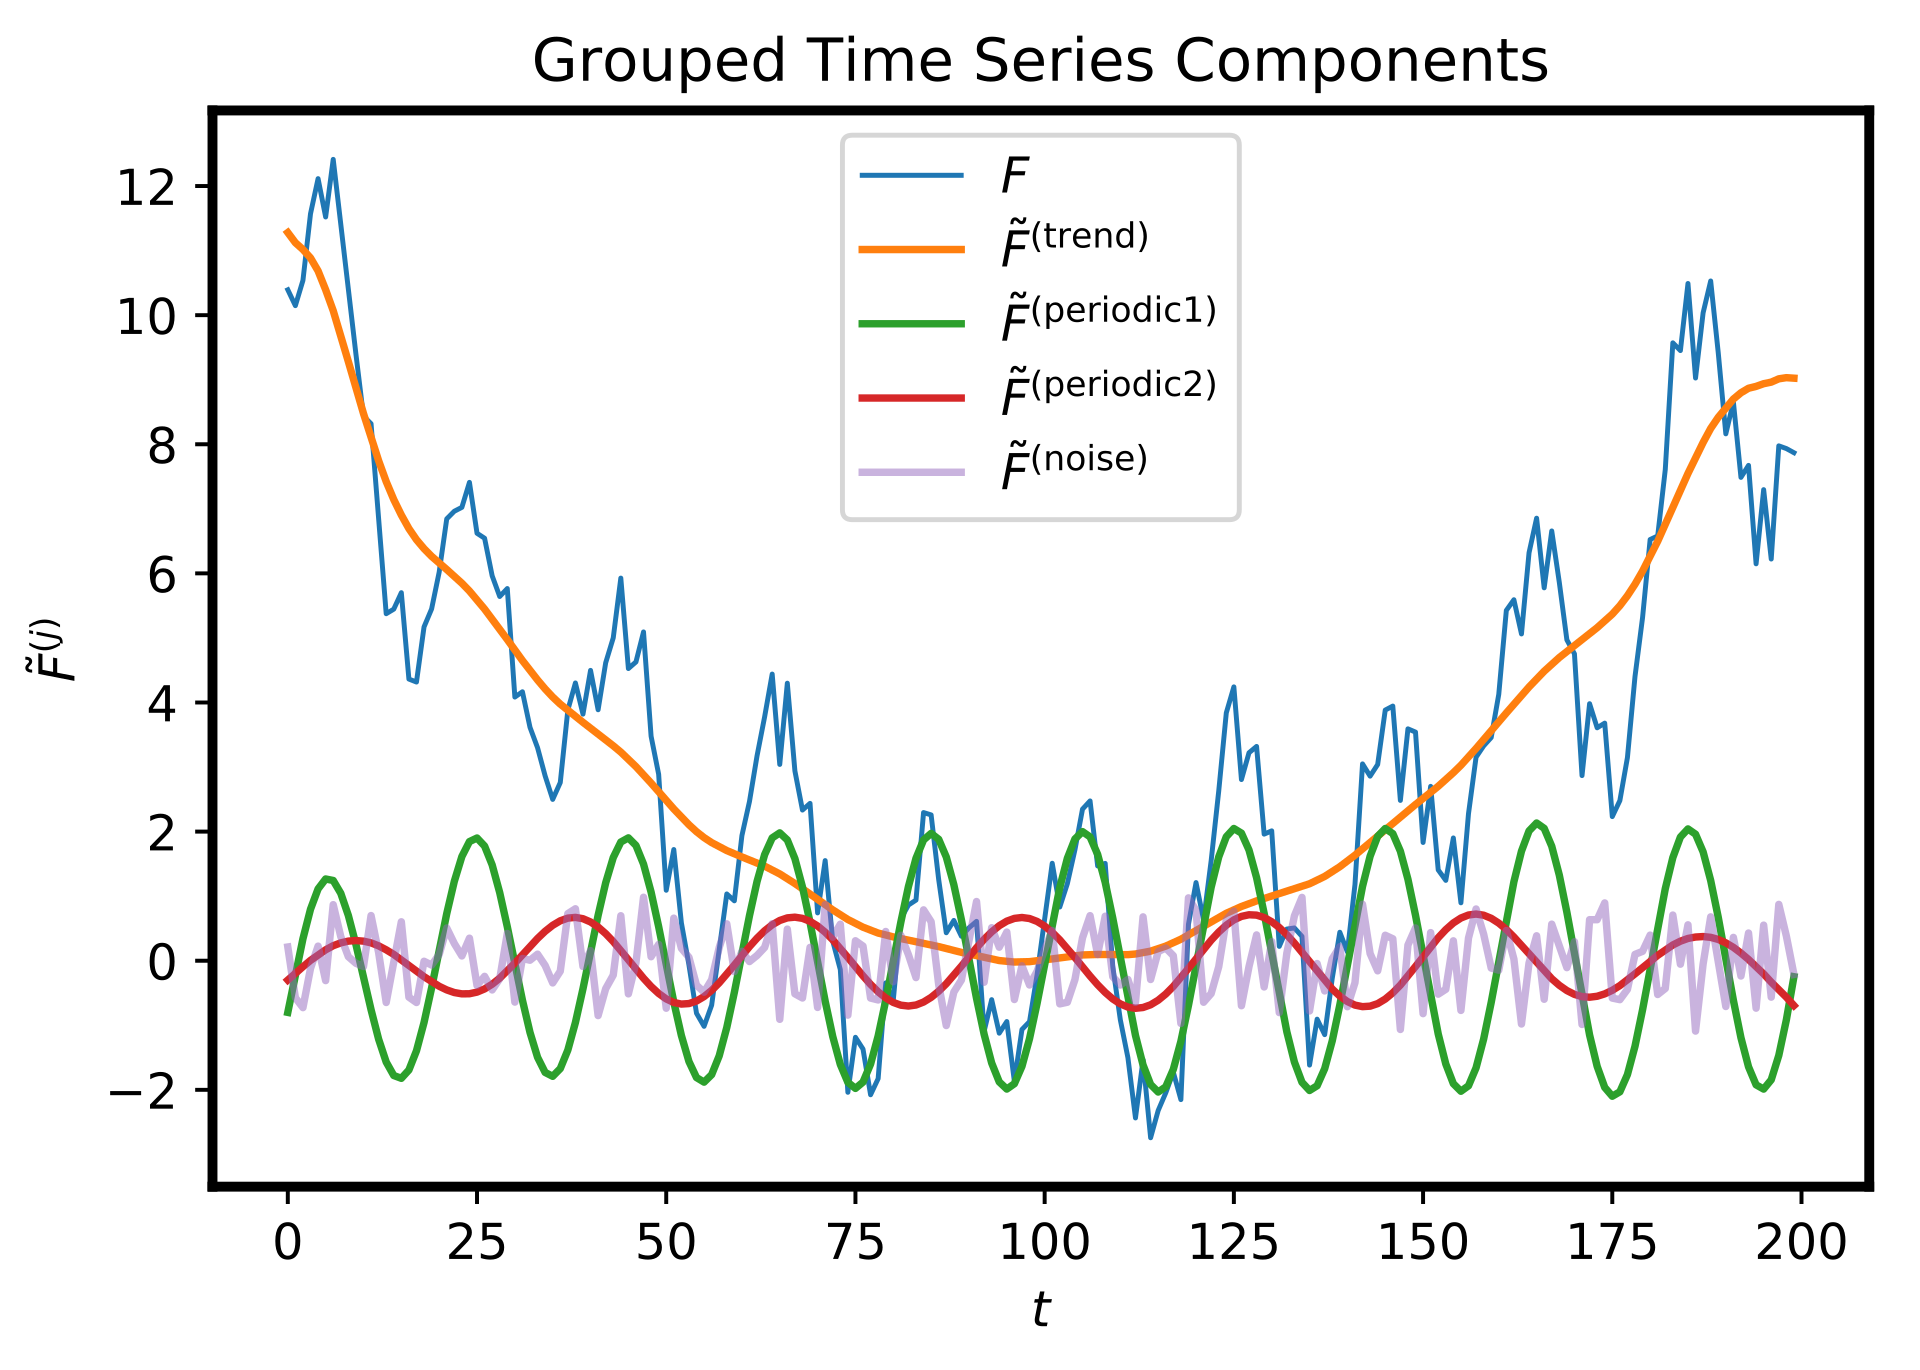
\includegraphics[width=0.9\textwidth]{lecture_14/figs/group_time_series.png}
\end{figure}
  
\end{frame}
%=======
\begin{frame}{Multivariate SSA}
Пусть имеется $P$ временных рядов $\{ x_t^{(1)} \}_{t=1}^T$, ...,  $\{ x_t^{(P)} \}_{t=1}^T$.
\begin{enumerate}
    \item Для каждого из рядов построим матрицу задержек $\M{X}^{(P)} \in \mathbb{R}^{\tau \times n}$.
    \item Объединим данные матрицы в одну 'длинную' блочную матрицу:
    $$ \M{X} = \Big(\M{X}^{(1)} \  \M{X}^{(2)} \ \dots \ \M{X}^{(P)} \Big) \in \mathbb{R}^{\tau \times Pn}$$
    \item Построим для объединённой матрицы задержек $\M{X}$ её низкоранговое приближение $\tilde{\M{X}}$.
    \item Получим сглаженные оценки элементов временных рядов $ \hat{x}_t^{(1)}$, ...,  $\hat{x}_t^{(P)}$ с помощью диагонального усреднения матрицы $\tilde{\M{X}}$, с учётом её блочной структуры.
\end{enumerate}
\end{frame}
%=======
\begin{frame}{Multivariate SSA}
\begin{figure}
    \centering
    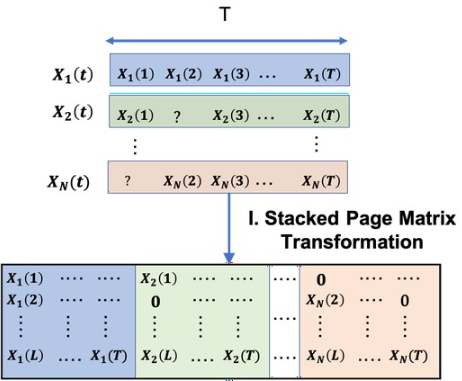
\includegraphics[width=0.8\textwidth]{lecture_14/figs/mssa_example.png}
\end{figure}
\end{frame}
%=======
\begin{frame}{Multivariate SSA. Сравнение с SSA}
\begin{figure}
    \centering
    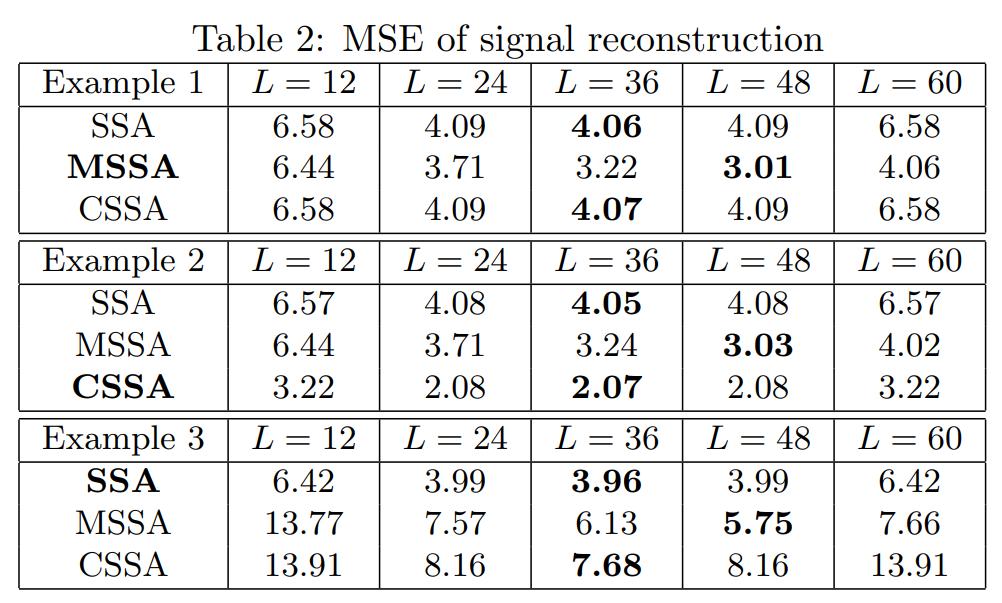
\includegraphics[width=0.8\textwidth]{lecture_14/figs/result_mssa.png}
\end{figure}
\myfootnotewithlink{https://www.gistatgroup.com/gus/mssa2.pdf}{сredit: Golyandina, N. and D. Stepanov (2005): "SSA-based approaches to analysis and forecast of multidimensional time series". In: Proceedings of the 5th St.Petersburg Workshop on Simulation, June 26-July 2, 2005, St. Petersburg State University, St. Petersburg, pp. 293–298}
\end{frame}
%=======
\begin{frame}{От mSSA к Tensor SSA для многомерного временного ряда}
\begin{itemize}
    \item Метод mSSA имеет преимущество, если временные ряды имеют совпадающие компоненты.
    \item Для учета более сложных зависимостей предлагается перейти от матричного вида к тензорному.
\end{itemize}

\noindent{
\begin{minipage}{.45\textwidth}
    \centering
    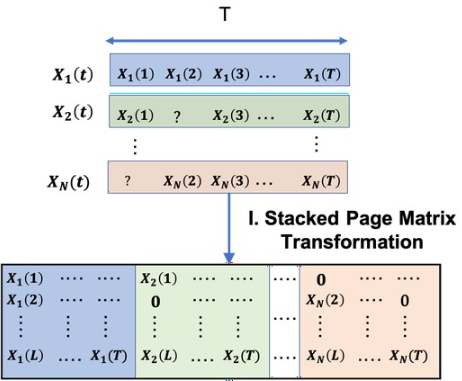
\includegraphics[width=0.9\textwidth]{lecture_14/figs/mssa_example.png}
\end{minipage}%
\begin{minipage}{.1\textwidth}
    \huge{\longrightarrow}
\end{minipage}%
\begin{minipage}{0.45\textwidth}
    \centering
    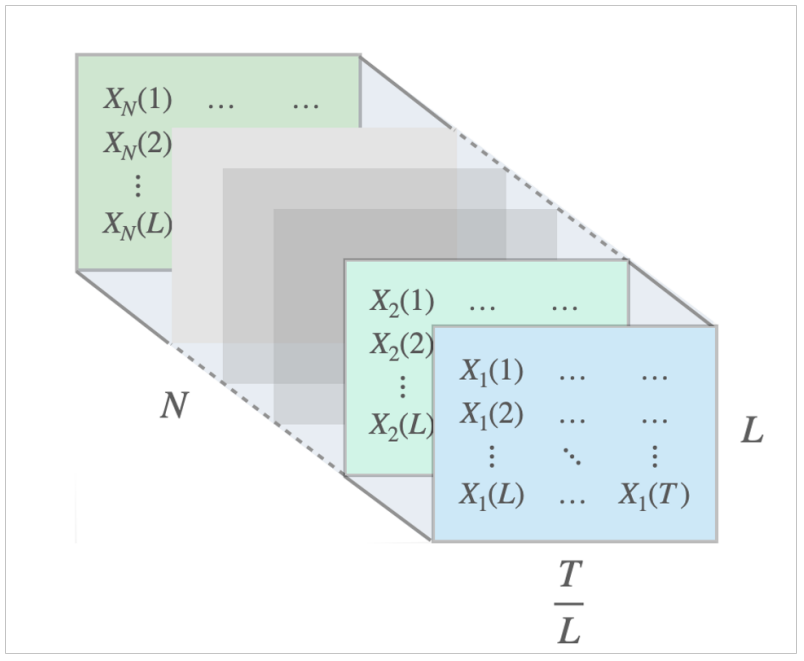
\includegraphics[width=0.9\textwidth]{lecture_14/figs/tensor_for_ssa.png}
\end{minipage}
}
\end{frame}
%=======
\begin{frame}{Tensor SSA}
Пусть имеется $P$ временных рядов $\{ x_t^{(1)} \}_{t=1}^T$, ...,  $\{ x_t^{(P)} \}_{t=1}^T$.
\begin{enumerate}
    \item Для каждого из рядов построим матрицу задержек $\M{X}^{(p)} \in \mathbb{R}^{\tau \times n}$.
    \item Объединим данные матрицы в тензор 3-его порядка:
    $$ \tensor{X}_{:, :, p} = \M{X}^{(p)}$$
    \item Построим для данного тензора приближение $\tilde{\tensor{X}}$ с помощью алгоритма ALS -- каноническое разложение ранга $R$ .
    \item Для срезов результирующего тензора $\tilde{\tensor{X}}_{:, :, p}$ осуществляем диагональное усреднение и получаем сглаженные оценки элементов временных рядов $ \hat{x}_t^{(1)}$, ...,  $\hat{x}_t^{(P)}$.
\end{enumerate}
\end{frame}

%=======
\begin{frame}{Tensor SSA для одномерного временного ряда}
\begin{figure}
    \centering
    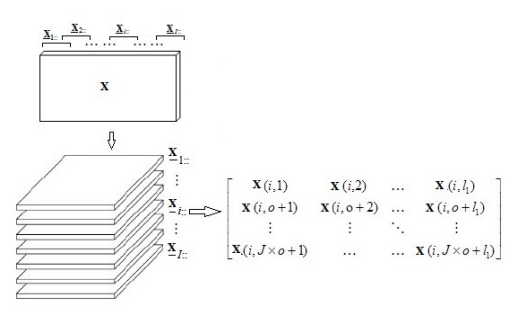
\includegraphics[width=0.75\textwidth]{lecture_14/figs/tSSA.png}
\end{figure}
\end{frame}

%=======
\begin{frame}{Tensor SSA. Сравнение с SSA}
\begin{figure}
    \centering
    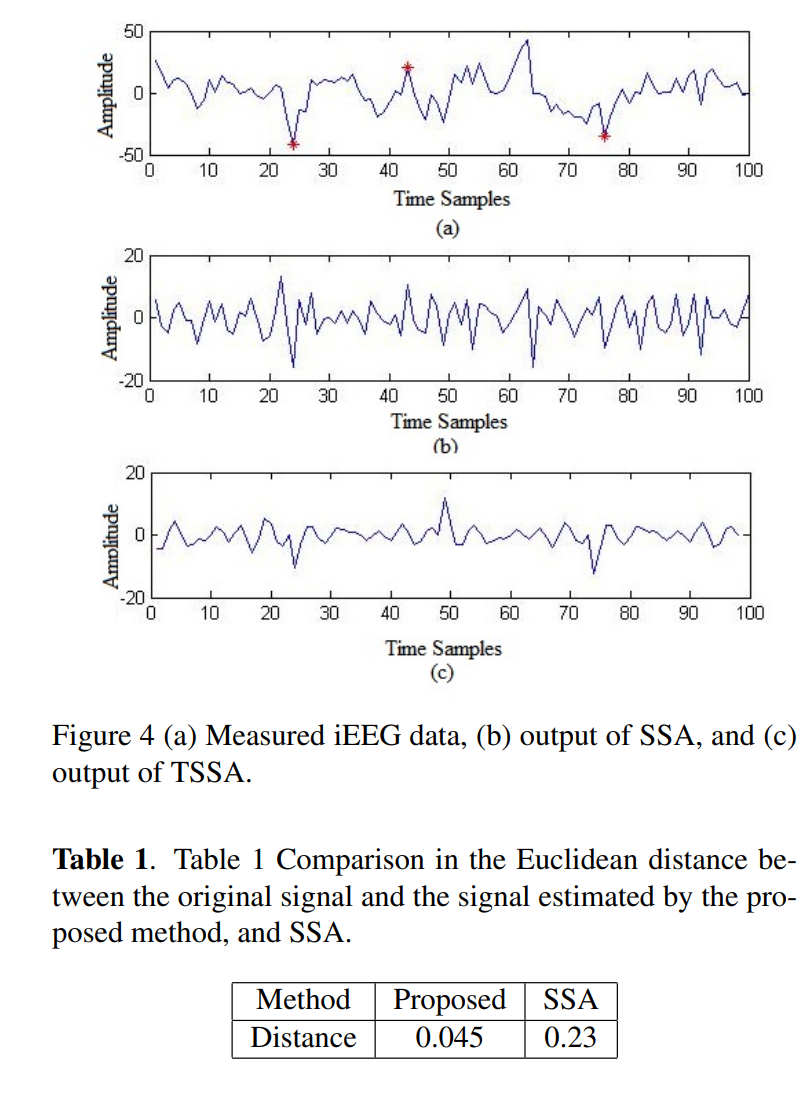
\includegraphics[width=0.4\textwidth]{lecture_14/figs/result_tssa.png}
\end{figure}
\myfootnotewithlink{https://ieeexplore.ieee.org/document/6661921}{сredit: S. Kouchaki and S. Sanei, "Tensor based singular spectrum analysis for nonstationary source separation," 2013 IEEE International Workshop on Machine Learning for Signal Processing (MLSP), Southampton, UK, 2013, pp. 1-5}
\end{frame}
%=======
\begin{frame}{Резюме}
\begin{itemize}
    \item SSA --- это связанный с SVD метод, который который позволяет разложить исходный  временной ряд на составляющие компоненты, сгладить, избавится от шума.
    \item В случае работы с многомерными временными рядами существует обобщение SSA --- mSSA.
    \item В mSSA используется матрица, полученная путем объединения ганкелевых матриц для каждого временного ряда.
    \item По аналогии с HOSVD SSA имеет обобщение на тензорный случай.
    \item С помощью CP-разложения выбираются интересующие компоненты, по аналогии с классическим SSA.
\end{itemize}
\end{frame}
\end{document} 